\newpage
%\thispagestyle{empty}
\mbox{}

\boldchapter{Dynamics of Nrd1-Nab3 RNA Binding \invitro{} and \invivo{}}

In chapter \ref{termination} I introduced the various termination pathways known in \cer{}. Among them, the NNS pathway is primarily responsible for termination of pervasive transcripts and a limited number of functional non-coding RNAs. Mechanistically, the NNS complex recognizes specific sequence elements on the nascent RNA and, once recruited, the subunit Sen1 is thought to translocate along the RNA and disassemble the elongation complex upon reaching it. 

Despite numerous studies, considerable doubt remains on what qualifies NNS terminators \invivo{}. Indeed, while the sequence elements bound by the members of the complex are known, no consistent patterns in number, disposition, or quality emerges from analysis of \invivo{} NNS terminators. 

Here we report preliminary analyses of an \invitro{} SELEX experiment performed with a purified Nrd1-Nab3 heterodimer in order to identify the main determinants of heterodimer binding. Additionally, we cross-reference these results with those of an \invivo{} SELEX experiment (Artificial CUT Selection) whose selection criteria is the efficiency transcription termination. In the context of these two experiments we find that particular arrangements and spacings between Nrd1 and Nab3 sites enhance binding efficiency \invitro{}, but not \invivo{}. Moreover, we identify several clusters of similar sequences that are differentially selected in the two experiments. Finally, we provide evidence that supports two distinct binding modes for nrd1 in binding its cognate sites GUAG and GUAA.



\singlespacing
\section{\Invitro{} Selection of RNA Sequences With High Affinity for the Nrd1-Nab3 Heterodimer}
\doublespacing

In order to determine the sequence elements with highest affinity for the Nrd1-Nab3 heterodimer, a SELEX experiment was performed in the laboratory by Jean-Baptiste Briand (Fig. \ref{fig:selex}A). 

\begin{figure}[h]

\centering
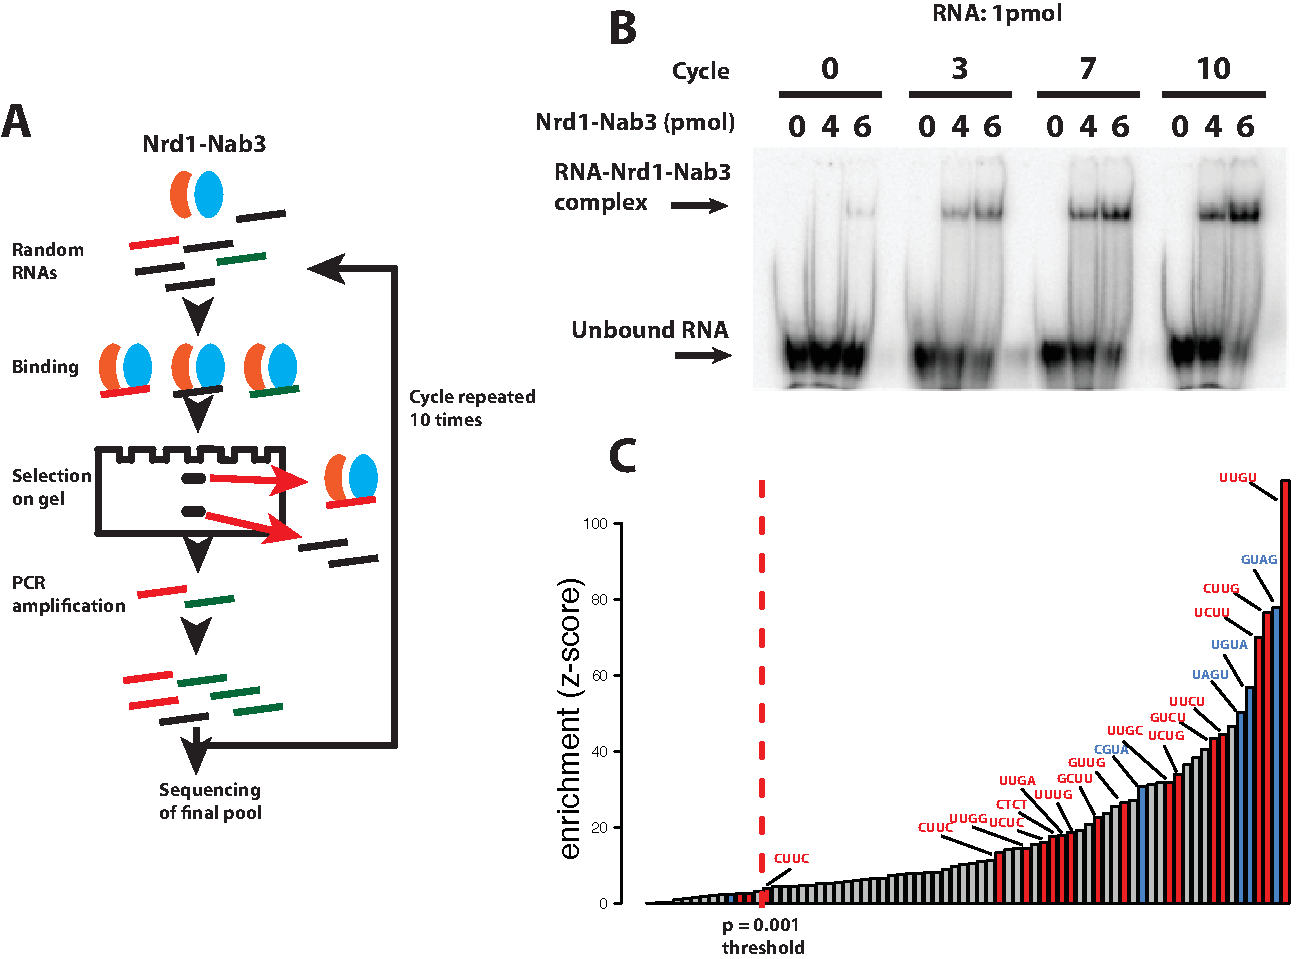
\includegraphics[width=\textwidth]{figures/results/selex}
\caption[SELEX procedure]{\textbf{A: }Schematic cartoon of the SELEX procedure. \textbf{B: }Electro Mobility Shift Assay (EMSA) performed with different protein concentrations and with sequence pools obtained after different number of SELEX cycles. As the cycles increase, the sequences are more likely to efficiently bind the heterodimer. \textbf{C: } Barplot displaying the most enriched motifs obtained through the SELEX procedure. Motifs with at least 3 nucleotides in common with the canonical Nab3 binding sites UCUUG are represented in red. Motifs with at least 3 nucleotides in common with the canonical Nrd1 binding sites GUA[A/G] are represented in blue.}
\label{fig:selex}

\end{figure} 

Full length, HIS-tagged Nrd1 and Nab3 were co-expressed and co-purified from E.coli, obtaining stable heterodimers. The recombinant heterodimer was then incubated with a naïve pool of chemically synthesized RNAs and retained only those that were bound to the Nrd1-Nab3 complex (fig. \ref{fig:selex}B). 
The selected RNAs underwent reverse transcription, PCR amplification, and \invitro{} transcription, yielding a new pool of sequences. The procedure was iterated for a total of 10 cycles and the final pool of high-affinity binders was submitted to deep sequencing,together with the original naïve pool. The 2000 most represented sequences in the final pool were retained for subsequent analyses. 



In order to evaluate the enrichment of specific motifs in the pool of selected sequences, we decided to adapt the Rsat algorithm for oligo-analysis \cite[see methods]{vanhelden:1998:extracting}. This procedure takes into account the nucleotide bias of the naïve pool, comparing the frequency of each motif in the background pool with that encountered in the selected pool and providing an enrichment score. As Nrd1 and Nab3 canonical binding sites have this length, we analysed all 4 nucleotide motifs.

As expected, we managed to identify a large number of known Nab3 and Nrd1 binding sites among the selected sequences (Fig. \ref{fig:selex}C). The canonical sites UCUU and GUAG were among the most enriched motifs, followed by close variants such as CUUG and UGUA. These results suggest that the pool of selected sequences contains high affinity bona fide binding sites for the Nrd1 Nab3 heterodimer. 

\singlespacing
\section{Arrangement of Binding Sites Influences Heterodimer Affinity \invitro{}}
\doublespacing

In order to determine whether efficiency of binding could depend on particular arrangements of Nrd1 and Nab3 sites, we analysed the enrichment of motifs containing different arrangements of Nrd1 and Nab3 sites separated by a variable number of random nucleotides. We analysed three canonical binding sites: Nrd1 binding sites GUAG and GUAA, as well as the Nab3 binding site UCUU.

\begin{figure}[hp!]

\centering
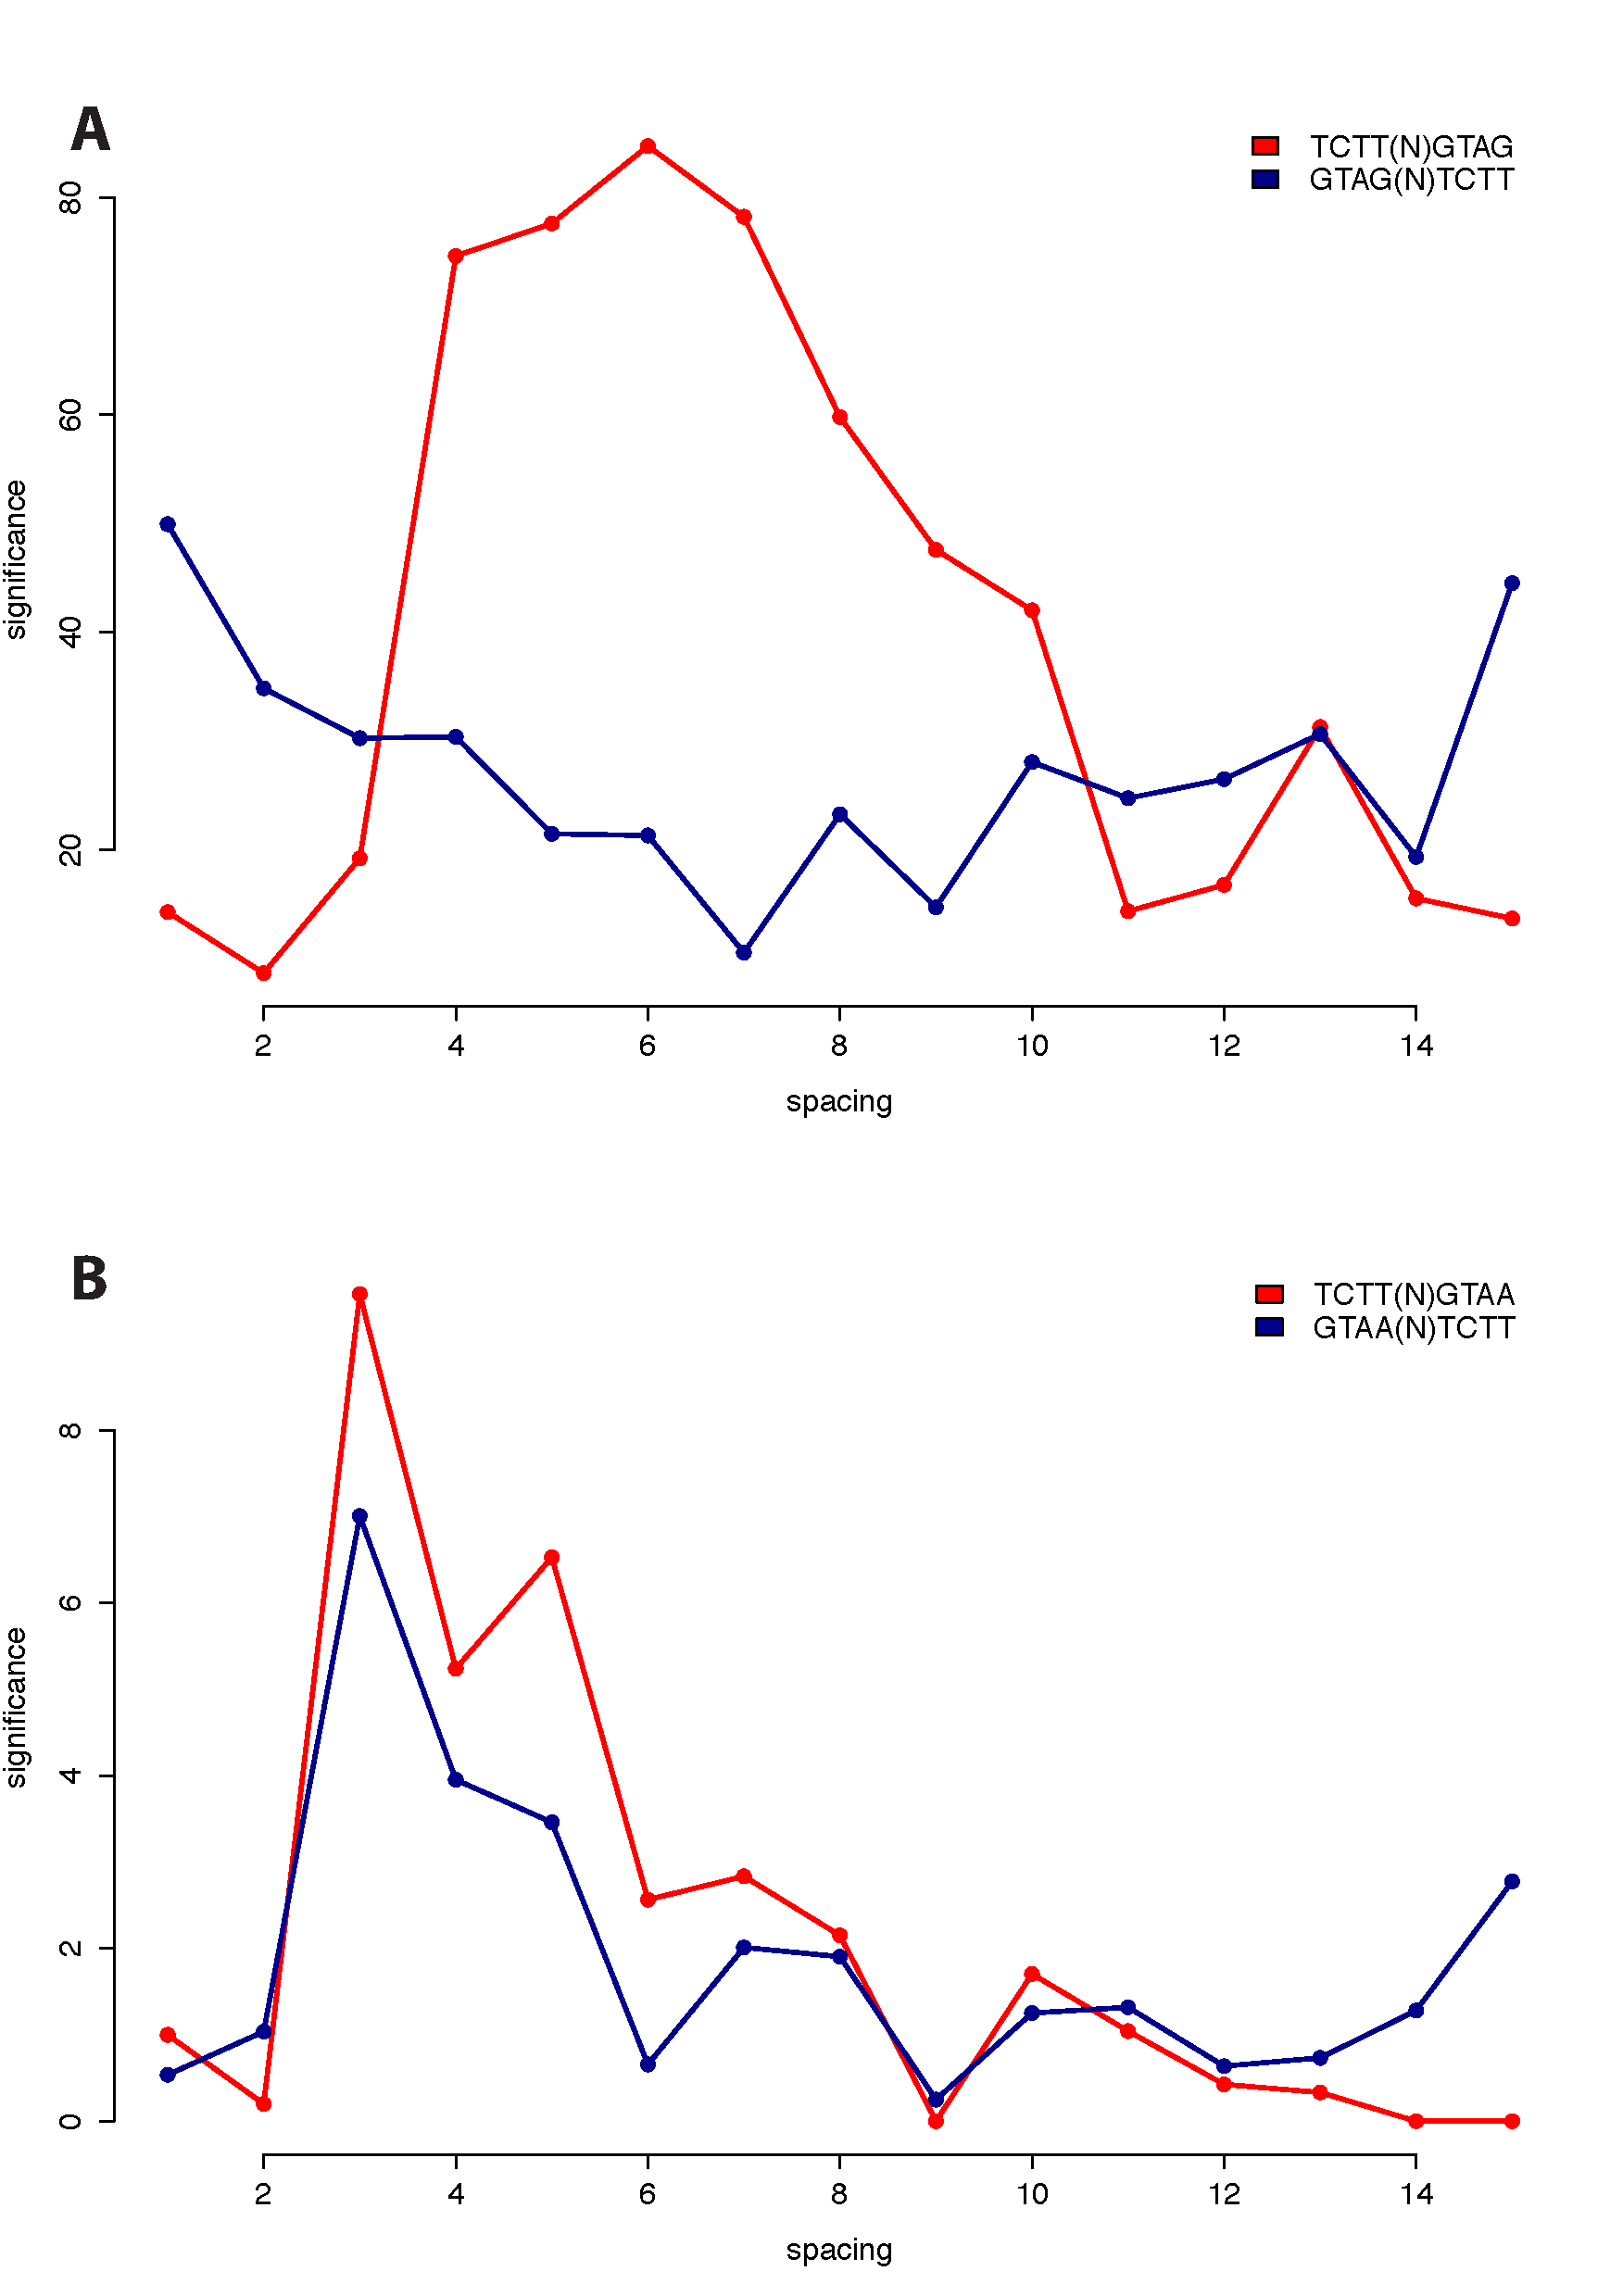
\includegraphics[width=\textwidth]{figures/results/positionalVitro}
\caption[Enrichment of Nrd1 and Nab3 sites with different arrangements and spacings in the SELEX experiment]{Significance of motifs with specific site arrangement and spacer length obtained from analysis of the SELEX experiment. Measures of significance were obtained by applying an adapted version of the Rsat algorithm \cite[see methods]{vanhelden:1998:extracting}.}
\label{fig:positionalVitro}

\end{figure} 

The plot in figure \ref{fig:positionalVitro}A shows motif enrichment as a function of spacing between Nab3 binding site UCUU and Nrd1 binding site GUAG.  We detect a marked increase in enrichment when UCUU and GUAG are separated by four to ten nucleotides, however, shorter or longer separators cause the significance of the enrichment to drop substantially. When the order of the sites was inverted (GUAG-N-UCUU), no such relationship could be observed. We repeated the same experiment using the Nrd1 binding site GUAA in place of GUAG (Fig \ref{fig:positionalVitro}B). Surprisingly, no pattern akin to the one we observed in figure \ref{fig:positionalVitro}A could be detected and both site arrangements show very similar enrichment patterns.

In order to assess the importance of these site arrangements within \invivo{} terminators, we decided to repeat these analyses on data coming from a previously published \invivo{} artificial CUT selection \cite{porrua:2012:in}. This strategy adopts the same principles of SELEX and allows screening a naïve pool of sequences for efficient termination \invivo{} (Fig. \ref{fig:vivoSelex}). The technique relies on a construct containing two strong promoters, pTET and pGAL, arranged in tandem and separated by a test sequence. While the first promoter drives transcription through the randomly selected sequence, the second controls the expression of the CUP1 gene, which allows yeast to grow on copper-containing plates. Transcription from the TET promoter will interfere with the expression of CUP1 unless the test sequence contains an efficient terminator, resulting in copper-sensitive yeast that will not grow on selective medium. After a naïve pool of chemically synthesised sequences was introduced in the construct, yeast underwent two rounds of selection on copper-containing plates. This led to sequencing of inserts containing NNS terminators. 

\begin{figure}[h]

\centering
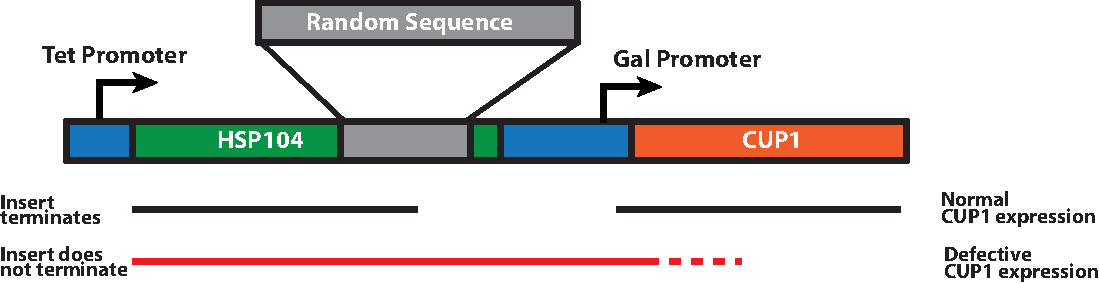
\includegraphics[width=\textwidth]{figures/results/vivoSelex}
\caption[Schematic of the selection process in the artificial CUT selection]{Cartoon showing the construct used to select sequences according to the efficiency of transcription termination in the artificial CUT selection. }
\label{fig:vivoSelex}

\end{figure} 

Because of the very similar nature of artificial CUT selection and classical SELEX experiments, results from both techniques could be analysed with the same statistical methods. The two assays, however, significantly differ in environment and selection criteria. While our SELEX experiment relies exclusively on \invitro{} binding of the isolated heterodimer to separate between selected and non-selected pools; artificial CUT selection requires the sequence to be an efficient \invivo{} terminator.  

The same analyses conducted on the \invitro{} SELEX winning pool were replicated on the pool of sequences obtained through the \invivo{} artificial CUT selection and are shown in figure \ref{fig:positionalVivo}. The enrichment patterns previously observed in fig \ref{fig:positionalVitro}A are not replicated in the artificial CUT selection. Spacing and arrangement analysis of UCUU and GUAG in the selected pool of \invivo{} CUT selection shows that no clear spacing-dependent pattern exists and that inverting the order of the sites has little effect. Analysis of UCUU and GUAA, however, reveals a striking alternating enrichment pattern that depends on both spacing and site arrangement (fig \ref{fig:positionalVivo}B). The length of the random spacers for which the UCUU-N-GUAA site arrangement is strongly enriched are also the ones for which GUAA-N-UCUU is poorly enriched. Vice versa, the spacer lengths for which GUAA-N-UCUU is strongly enriched, result in poor enrichment when sites are inverted. 

Taken together, these results suggest that particular dispositions and spacing of GUAG, GUAA, and UCUU binding sites can affect the binding affinity of the Nrd1-Nab3 heterodimer and possibly its efficiency in eliciting termination. 

\begin{figure}[hp!]

\centering
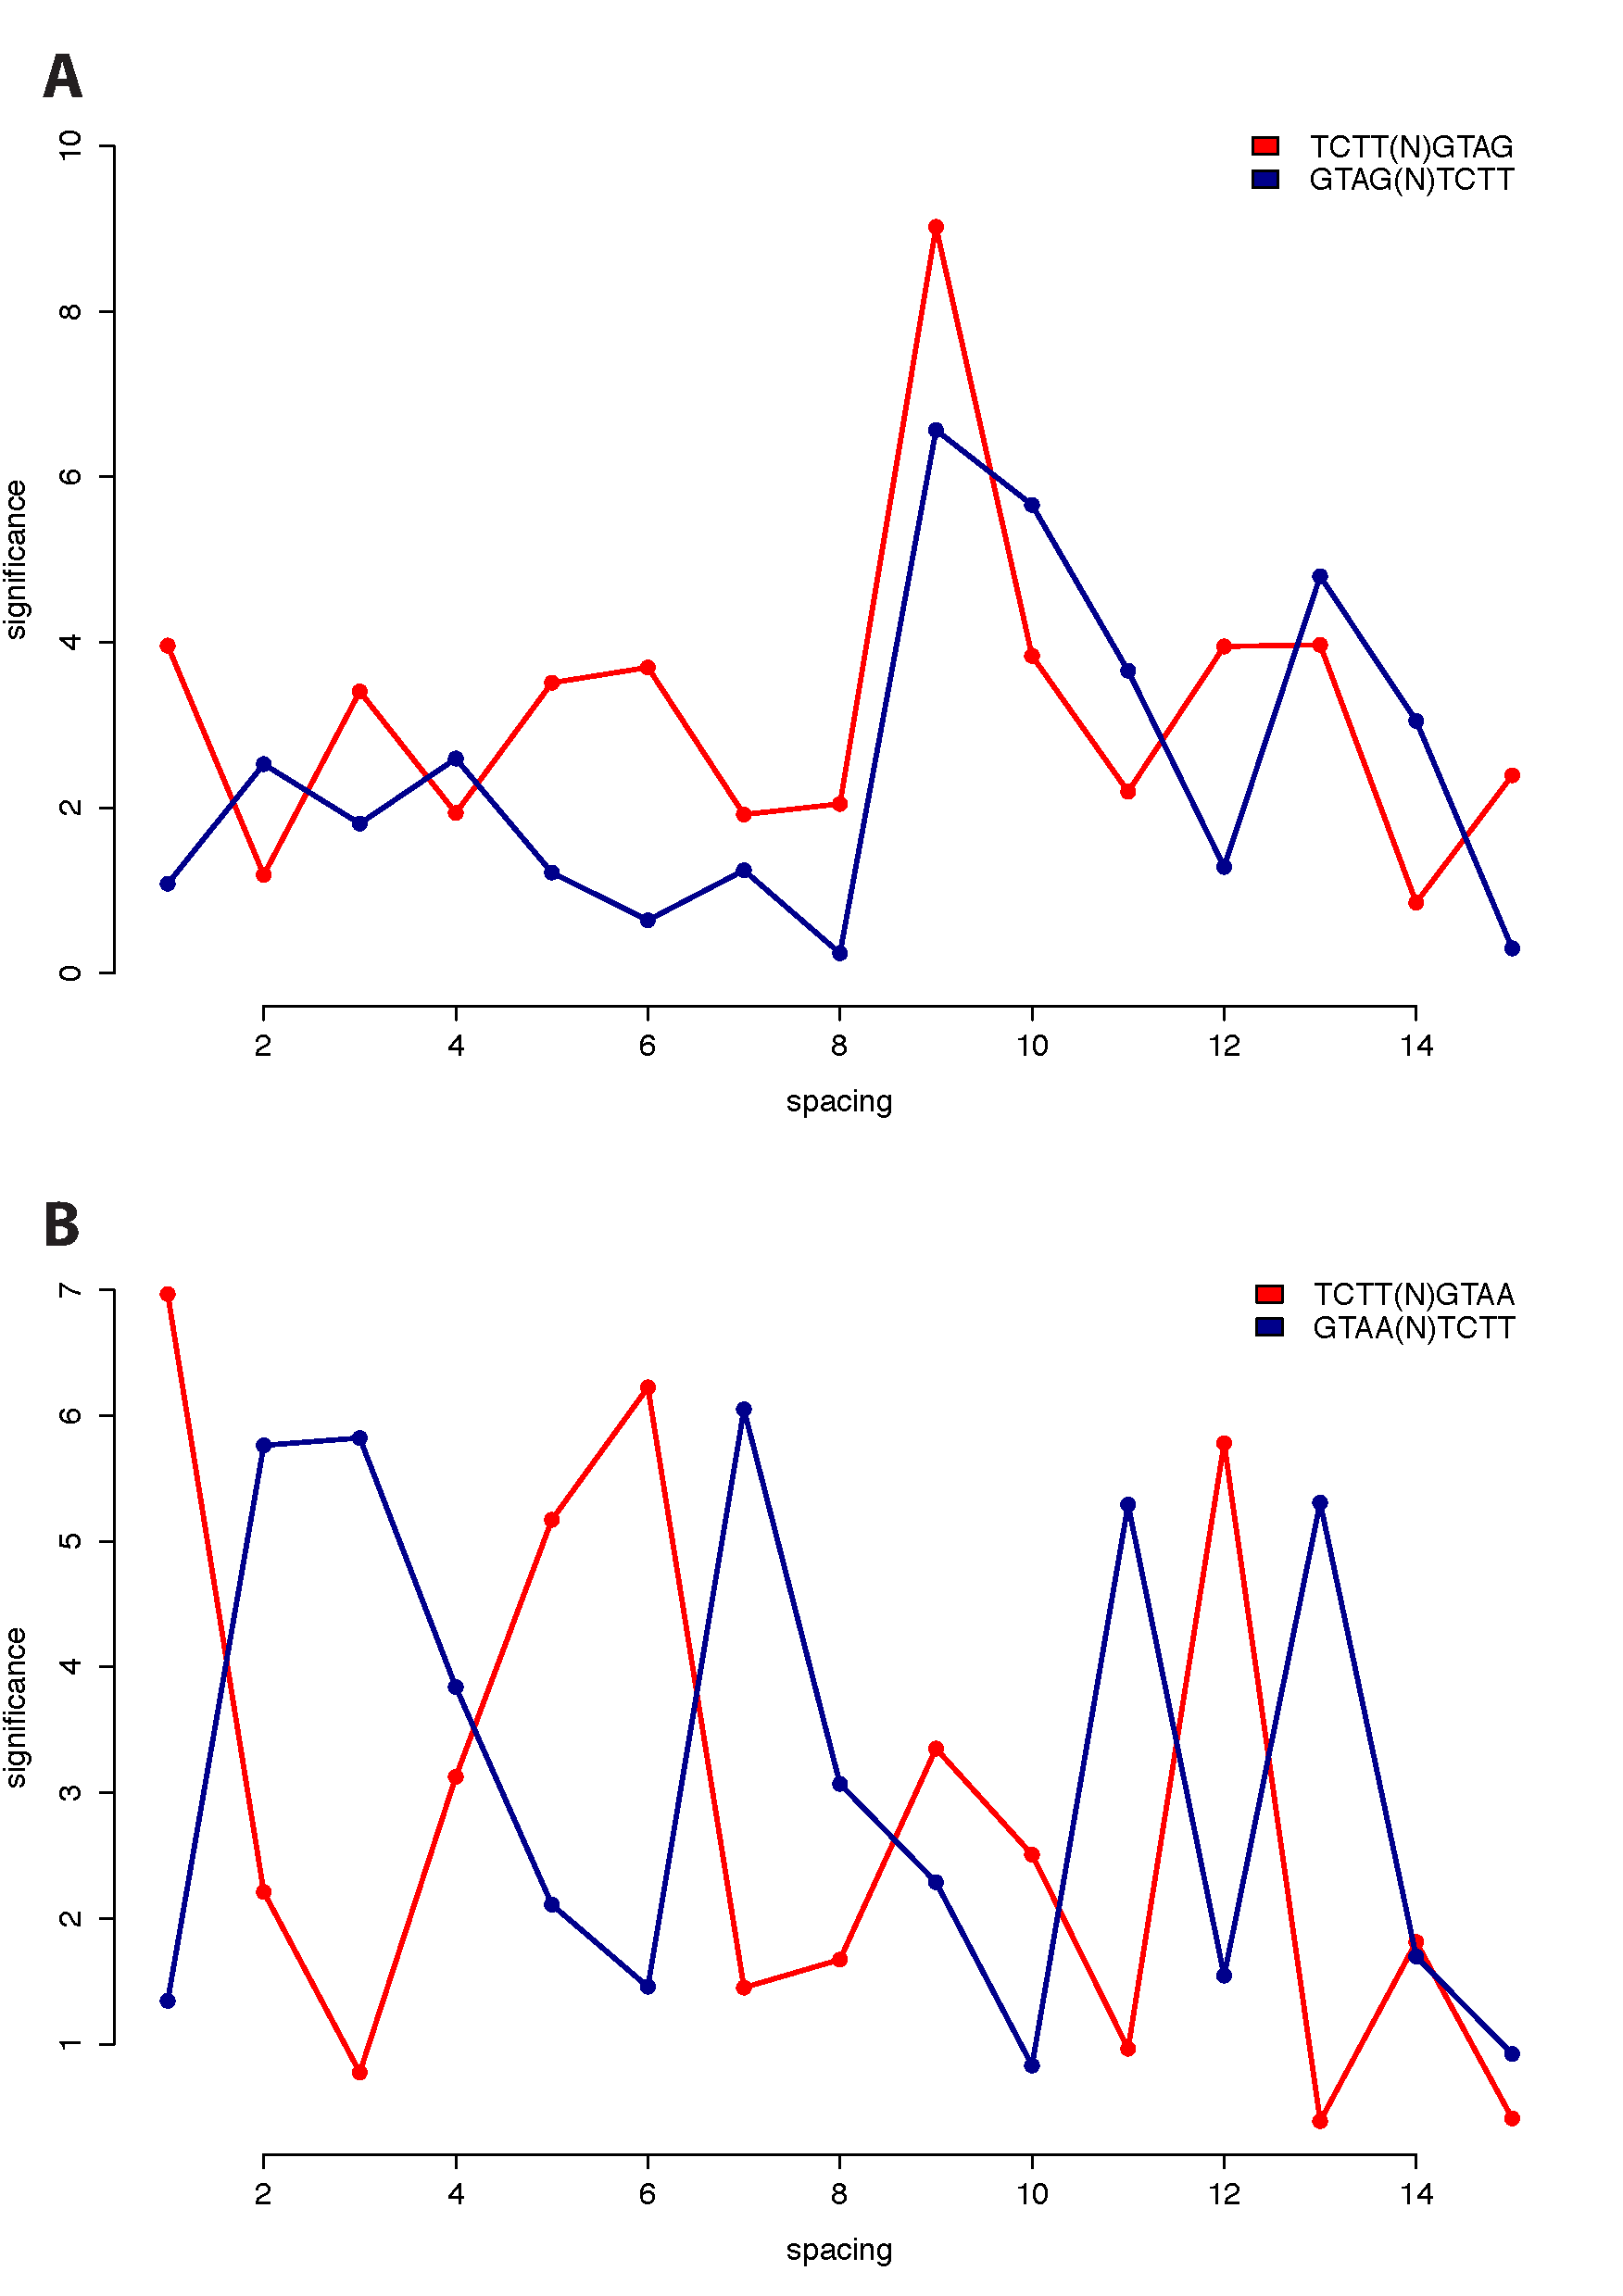
\includegraphics[width=\textwidth]{figures/results/positionalVivo}
\caption[Enrichment of Nrd1 and Nab3 sites with different arrangements and spacings in the artificial CUT selection]{Significance of motifs with specific site arrangement and spacer length obtained from analysis of the artificial CUT selection. Measures of significance were obtained by applying an adapted version of the Rsat algorithm \cite[see methods]{vanhelden:1998:extracting}.}
\label{fig:positionalVivo}

\end{figure} 

\singlespacing
\section{Comparison of SELEX and \invivo{} artificial CUT selection unveils unexpected dynamics of Nrd1 binding}
\doublespacing
In order to obtain a clearer view of the differences between \invitro{} SELEX (RNA binding as selection criterion) and artificial CUT selection (terminator efficiency as selection criterion) we performed motif enrichment analysis and plotted enrichment significance for both experiments (Fig. \ref{fig:selexComp}A), setting a confidence threshold at $p$ = 0.001. As expected, the two experiments partially correlate (Pearson's $r$=0.44). This reflects the relationship between binding of the NNS complex to the RNA and subsequent termination. Interestingly, however, several clusters of similar sequences were differentially enriched (fig. \ref{fig:selexComp}B). 

Nab3 binding sites and their variants, along with UC-rich sequences, were strongly selected in both experiments. This is consistent with previous reports that frame Nab3 binding as the most important contributor to overall heterodimer binding affinity.

Heavily G-rich sequences, conversely, were strongly counter-selected in both experiments. This provides evidence that both in the context of the Nab3-Nrd1 heterodimer and \invivo{}, G-rich sequences do not favour binding  or termination by the NNS complex.

AU-rich sequences were found to be prevalent both in natural cases and in the artificial CUT selection experiment and were shown to enhance Nrd1 binding \cite{porrua:2012:in}. Surprisingly, AU-rich sequences were not enriched in our SELEX experiment and their frequency is significantly lower than expected by chance. A similar but opposite trend was detected for GU-rich sequences. These were enriched in the SELEX experiment, but were counter-selected in the artificial CUT selection. 

Interestingly, the enrichment of canonical Nrd1 binding sites in the two experiments mirrors that of GU-rich and AU-rich sequences. In our SELEX experiment, the more G-rich site, GUAG, was by far the most enriched Nrd1 binding site, but was only moderately enriched in the artificial CUT selection (SELEX enrichment $p$ $<$ 1E-100, CUT selection enrichment $p$ = 1.9E-3). 
\begin{figure}[h!]

\centering
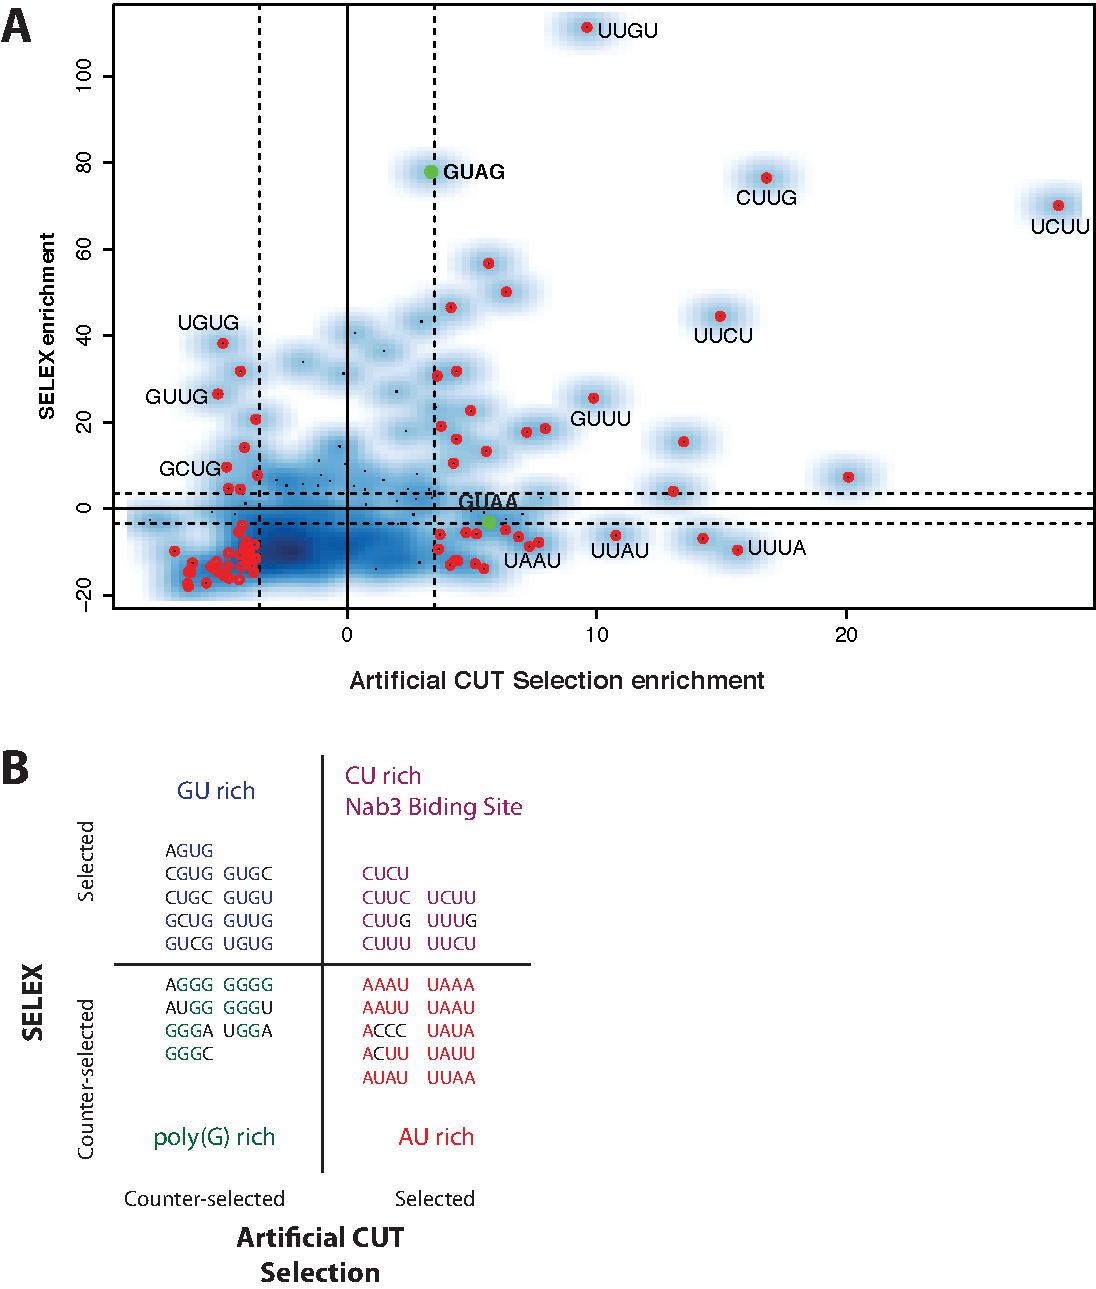
\includegraphics[width=\textwidth]{figures/results/selexComparison}
\caption[Direct enrichment comparison between SELEX and artificial CUT selection for all 4 nucleotides motifs]{\textbf{A: }Scatterplot of SELEX vs artificial cut selection enrichment for all 4 nucleotide motifs. Dashed lines represent $p$ = 0.001 confidence intervals. Significant sequences are highlighted in red. \textbf{B: }A schematic view of the enriched and depleted sequences between the two experiments.}
\label{fig:selexComp}

\end{figure} 
Conversely, GUAA is the most prominent Nrd1 binding site identified in the artificial CUT selection, while it is counter-selected in the SELEX (SELEX enrichment $p$ = 0.99, CUT selection enrichment $p$ = 1.1E-7). 



Taken together these results confirm the important role of Nab3 as the main contributor to NNS specificity both \invivo{} and \invitro{} and unveil an unexpected dynamic of Nrd1 binding sites selection depending on both context and type of selective pressure.

\singlespacing
\section{Nrd1 Binding Sites GUAG and GUAA Possess Different Extended Consensuses}
\doublespacing

Nrd1’s differential affinity for its two major binding sites poses questions regarding its mode of binding. Recent studies proposed that Nrd1’s RRM is bipartite, one part has high affinity for AU-rich sequences, while the other prefers GU-rich sequences \cite{bacikova:2014:structure}. According to this study, the two binding surfaces are semi-independent and mutations on one part has only minor effects on the other part’s ability to contact its cognate sites. 

In order to test the hypothesis that GUAA and GUAG might require two different binding modes, we decided to explore whether these two core motifs have the same preference for flanking nucleotides. Different preferences would indicate that [A] and [G] at position four in the consensus are not simply interchangeable, but impact the conformation of Nrd1 binding to the site.

To achieve this, we measured the nucleotide frequency before and after each of the sites in the SELEX and compared it with the overall nucleotide frequency in the pool of selected sequences. 
This allowed us to quantify the nucleotide distribution and to determine their over- or under-representation relative to their abundance in the rest of the pool (see methods).
Log$_2$ of the ratio between the nucleotide frequency flanking Nrd1 sites and the overall frequency in the datasets are shown in figure \ref{fig:flanking}A, positive values imply an enrichment around the Nrd1 site, while negative values indicate a depletion, stars indicate a statistically significant depletion or enrichment based on the binomial test (see methods).

Direct comparison of the extended consensuses for these two core Nrd1 binding sites reveals substantial differences. While presence of a G before or after both sites is universally counter-selected, its presence before GUAG is about 10 fold less likely than in the case of GUAA. The two binding sites also substantially differ in their preferences for both preceding and following As. As are heavily enriched following GUAA, while in GUAG only a minor enrichment is detected in this position, giving preference to Us, which are depleted in GUAA. 

\subsection{Confirming the Differences \invivo{}}

The stark differences we detected between the two major Nrd1 binding sites in our SELEX experiment prompted us to verify this relationship \invivo{}. To achieve this, we decided to apply the same technique to a pool of CUT sequences extracted from the genome (Fig. \ref{fig:flanking}B). CUTs represent the major fraction of NNS terminated non-coding RNAs and are therefore good candidates to test our hypothesis.

\begin{figure}[h!]

\centering
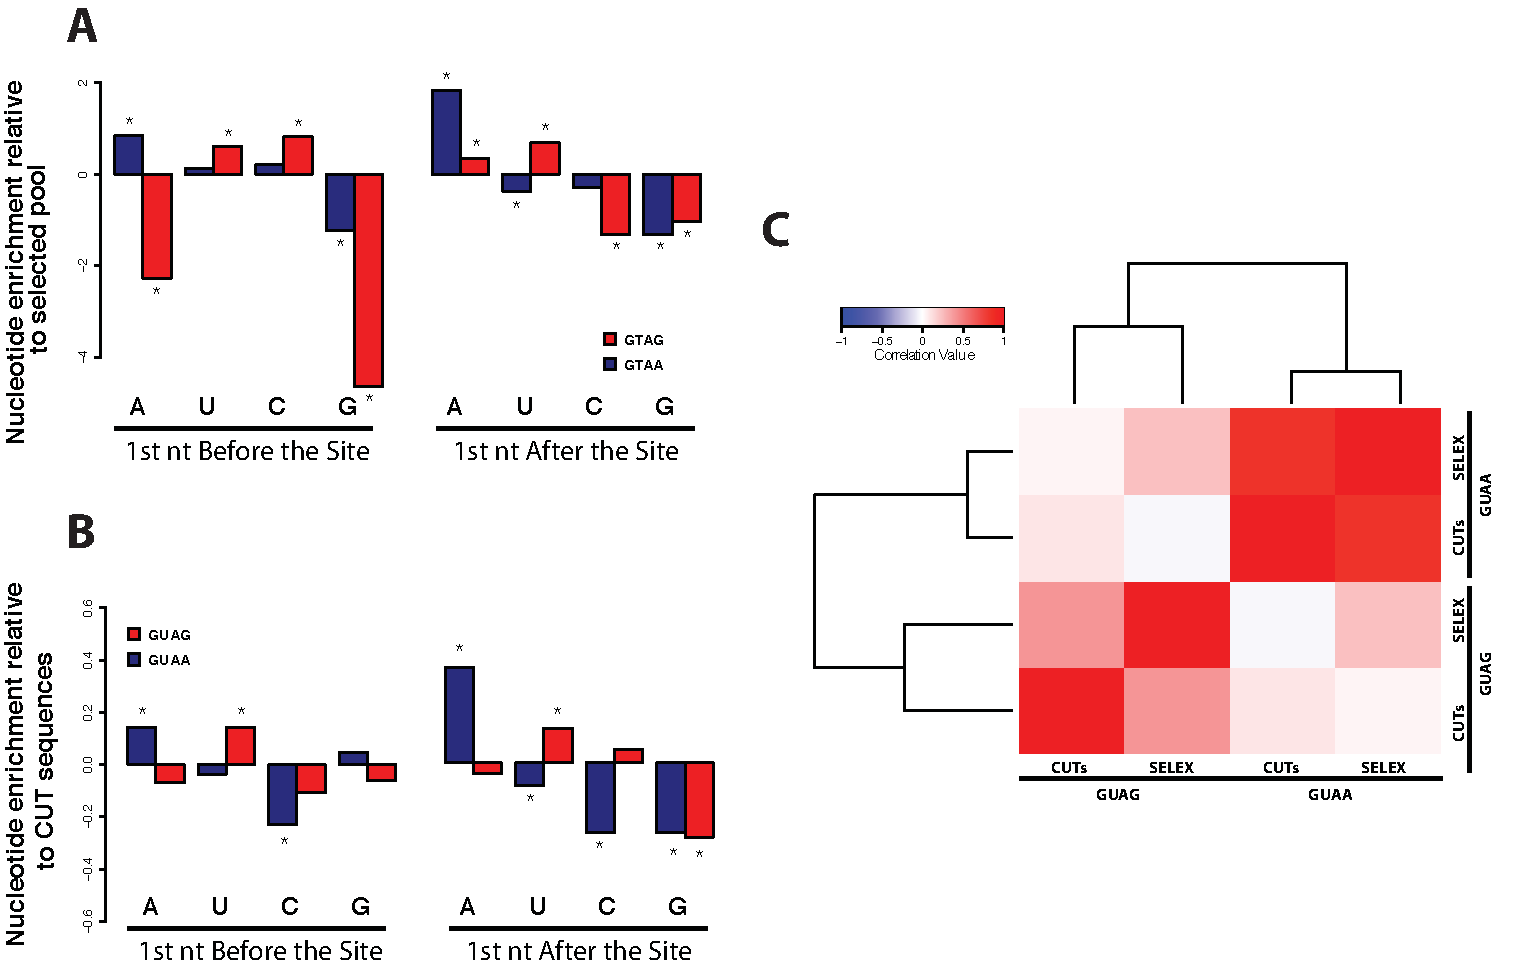
\includegraphics[width=\textwidth]{figures/results/gtagGtaaFlanking}
\caption[Comparison of flanking nucleotides between GUAG and GUAA in SELEX and genomic CUT sequences]{\textbf{A and B: }Representation of the comparative enrichment of every nucleotide before and after Nrd1 binding sites GUAG and GUAA.  \textbf{C: }Heatmap of pairwise Pearson's correlation values between every site-dataset combination. Binding sites prove to correlate well with themselves irrespective of datasets, while different binding sites poorly correlate.}
\label{fig:flanking}

\end{figure} 

As described previously, we analysed the nucleotide frequencies of the position preceding and following the two major Nrd1 binding sites: GUAG and GUAA. The two sites show distinct patterns that globally mirror what was observed in the analysis of the SELEX sequences, although the differences are less stark. GUAA is still significantly associated with As, both in the preceding and following position while GUAG prefers Us. In addition to the similarities, we observed some differences between nucleotide frequencies in CUTs and in the SELEX sequences. Presence of a G before both Nrd1 sites does not seem to be as depleted in CUTs as it is in the SELEX sequences; also, presence of A preceding GUAG seem to be better tolerated in CUTs. 

In order to assess the similarity between patterns of nucleotide enrichment across different binding sites and datasets, we decided to perform pairwise correlations. Each combination of site and dataset (e.g. GUAA in CUT sequences) was associated with 8 numerical values corresponding to the relative frequencies of flanking nucleotides (A, T, G, or C, before and after the site).  We then calculated the Pearson’s correlation between each site-dataset pair. Figure \ref{fig:flanking}C shows that pairwise correlation between GUAG and GUAA is very low irrespective of which dataset is used to carry out the analysis. Conversely, SELEX sequences and CUTs agree well on the trend in nucleotide enrichment for the two sites.

Taken together, these results indicate that the extended consensus of the two main Nrd1 binding sites GUAG and GUAA differ substantially both \invitro{} and \invivo{}. This might suggest that Nrd1 has different binding modes depending on the site that is contacted, supporting the hypothesis of a bipartite RRM.

\clearpage

\section{Discussion}

In this work, we investigated the binding of the Nrd1-Nab3 heterodimer to its cognate sites in the context of two techniques: an \invitro{} SELEX experiment whose selection criteria is binding; and an \invivo{} CUT selection experiment selecting for sequences able to terminate transcription. We found that a particular arrangement and spacing of UCUU and GUAG sites is strongly enriched in the SELEX experiment, but this enrichment is not mirrored in the CUT selection experiment. Conversely, we found that the sites UCUU and GUAA display a peculiar alternating enrichment pattern in the \invivo{} CUT selection, while no such pattern could be detected in the SELEX experiment.

At the same time, we compared enrichment of 4 nucleotide motifs in both experiments and analyzed clusters of similar sequences across the two experiments. We found that Nab3 sites (and CT-rich sequences in general) are strongly enriched in both experiments, while G-rich sequences are counter-selected for both \invitro{} binding and \invivo{} termination. Additionally, we found that AU-rich sequences---already known to enhance Nrd1 binding and termination \invivo{} \cite{porrua:2012:in}---were enriched in the CUT selection, but strongly depleted in our SELEX experiment. Conversely, GU-rich sequences were strongly selected in the selex experiment, but counter-selected in the \invivo{} CUT selection. Curiously, we observed that two versions of the Nrd1 binding site consensus were also following this pattern. Nrd1 site GUAG is strongly enriched in the SELEX and significantly less so in the CUT selection, while GUAA was depleted in the SELEX and strongly enriched in the CUT selection. 

We speculate that, depending on the environment and selective pressure, Nrd1 would have higher affinity either for GU-rich sequences or AU-rich sequences and that this altered affinity would be reflected in the choice of binding site: GUAG in the former case, GUAA in the latter. This notion is supported by a recent study where Nrd1 is shown to possess a bipartite RRM that can shift to accommodate either AU-rich sequences or G-rich sequences, potentially resulting in two different binding modes \cite{bacikova:2014:structure}.  To test the hypothesis that GUAG and GUAA might trigger two different binding modalities in Nrd1, we analyzed the frequency of nucleotides flanking these two motifs both in our SELEX experiments and in CUT sequences extracted from the genome. We found that GUAG and GUAA have different preferences for flanking nucleotides and possibly different extended consensuses. Pairwise correlation analyses between different datasets and different binding sites reveal that the frequency of flanking nucleotides relative to the background remains similar across datasets, but not across binding sites.

\singlespacing
\subsection{Site Arrangement and Spacing Influence Binding Affinity and Termination Efficiency}
\doublespacing

Our SELEX experiment coupled with the Rsat algorithm for statistical analysis \cite{vanhelden:1998:extracting} allowed us to determine an enrichment score over the background pool for any sequence. We therefore decided to explore the effect of random nucleotides separating Nrd1 and Nab3 sites on their overall binding affinity. Strikingly, Nab3 site UCUU followed by a spacer of 4-10 nucleotides and then followed by the Nrd1 site GUAG proved to be highly enriched, substantially more that the same sequences spaced by 1-3 or 11+ nucleotides.

We speculate that 4-10 nucleotides represents the most accommodating spacing for the cooperative binding of the heterodimer: a shorter spacing could lead the two proteins to sterically or otherwise interfere with one another, while a longer one would lead the two sites to be bound independently and not cooperatively because of the excessive distance. In our analyses, we also noticed that swapping the sites of Nrd1 and Nab3 did not result in a similar enrichment. This suggests that binding is directional, and that the heterodimer can effectively bind both a Nrd1 and Nab3 site at the same time only if they are present in a particular order. However, it is possible that these enrichment patterns only hold \invitro{} or under these particular conditions, as we found no \invivo{} evidence of this arrangement being preferred.

Another perplexing finding regards the results of this experiment when performed on the alternative Nrd1 binding site GUAA. While we could not detect any noteworthy pattern when UCUU-N-GUAA is analysed in the context of the SELEX experiment, the same analysis performed on the artificial CUT selection resulted in a striking alternating pattern that depends on both site arrangement and spacer length. At this stage it is difficult to speculate on a reason that would cause this pattern would emerge. However, we think that a fundamental difference in the binding mode of Nrd1 to its cognate sites GUAA and GUAG could affect the overall binding patterns of the heterodimer. Alternatively, we must consider the caveat that SELEX and artificial CUT selections are widely different experiments and that technical or indirect effects could play a substantial role in influencing sequence enrichment dynamics. 

\singlespacing
\subsection{Comparison of SELEX and \invivo{} CUT Selection Reveals Clusters of Differentially Enriched Sequences}
\doublespacing

We compared the enrichment of all 4 nucleotide motifs in the SELEX and \invivo{} CUT selection and analyzed which clusters of sequences were enriched or depleted in both experiments, as well as determining the differentially enriched sequences. Because of the different environment and selection criteria for these two experiments, we could speculate on the role that each of these sequence clusters. 

We found that UC-rich sequences---among which the Nab3 binding consensus features prominently---were universally enriched in both experiments. This result is consistent with the role of Nab3 in NNS termination, as well as previous reports that put Nab3 binding as the main contributor to heterodimer binding \cite{carroll:2007:interaction}. Second, we found that heavily G-rich sequences were counter-selected in both experiments. Because G-rich sequences are not conducive to Nab3 binding and, to a lesser extent, to Nrd1 binding, we propose that these sequences are not competent for heterodimer binding, and therefore cannot elicit termination, resulting in a depletion in both experiments. Finally, we found that AU-rich sequences were selected in the CUT selection, but counter-selected in the SELEX, while GU-rich sequences followed the opposite trend, being enriched in the SELEX but counter-selected in the CUT selection. It is tempting to speculate that AU-rich sequences could be required only for termination and not for binding, however, this leaves open the question of why GU-rich sequences are selected for binding \invitro{}, but not for termination \invivo{}. Another possibility is that Nrd1 could differentially interact with these sequences in the two experiments. Previous \invitro{} studies reported that Nrd1 possesses two different binding domains, one with high affinity for G-rich sequences, and with high affinity for AU-rich sequences. We speculate that these two binding domains have different binding modes and binding strengths. The evidence we found is consistent with a model where Nrd1 GU-binding domain is stronger than the AU-binding domain, leading to counter-selection of AU-rich sequences in the SELEX experiment, where heterodimer binding is the only selection criteria. Conversely, we speculate that the AU-rich binding mode, although weaker, is somehow more conducive to transcription termination, possibly due to structural rearrangements that facilitate the process. 

In order to further support this model, we tested whether GUAG (enriched in SELEX) and GUAA (enriched in CUT selection and in CUT sequences \invivo{}) had different preferences for flanking nucleotides. This would suggest that GUAG and GUAA are not merely two alternative versions of the same consensus, but make a different set of contacts with Nrd1’s RRM. Our results support this view, as the two sites display different flanking nucleotide preferences both in the SELEX experiment and in CUT sequences extracted from the genome. 




